\newpage
\section{Resultados}
\label{sc:resultados_}

{
A partir da plotagem dos gráficos referentes aos valores de tensão armazenados no cartão SD, foram extraídas as conclusões iniciais. No gráfico presente na figura \ref{fig:grafico_results_01}, percebe-se uma relativa aproximação com os valores teóricos, cuja a divergência foi o fator da descarga da bateria acontecer de forma exponencial, de maneira a impossibilitar os cálculos teóricos exatos.
}

\begin{figure}[htp]
    \centering
    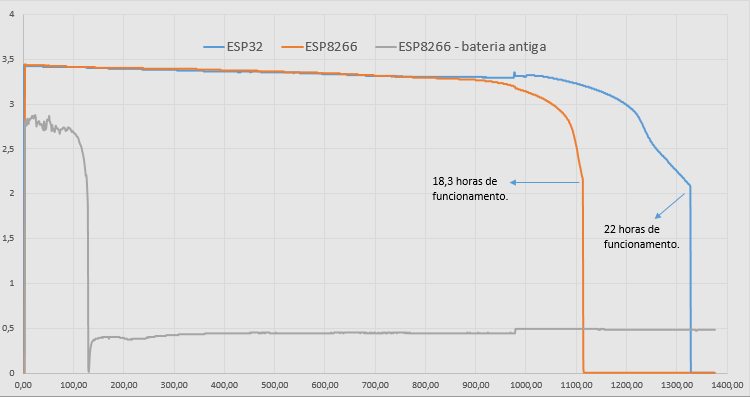
\includegraphics[scale = 0.8]{Graficos/grafico_01.png}
    \caption{Gráfico 1 - Teste sem troca de funções}
    \label{fig:grafico_results_01}
\end{figure}

{
Com base na análise do gráfico 2 de consumo – figura \ref{fig:grafico_results_02}, percebe-se a presença de várias variações bruscas de tensão, esse fato se deve ao modo de funcionamento em que as placas ESPs foram pré-programadas, pois com a troca do modo de operação, ocorre a troca de intensidade do consumo de corrente elétrica. 
}

\begin{figure}[htp]
    \centering
    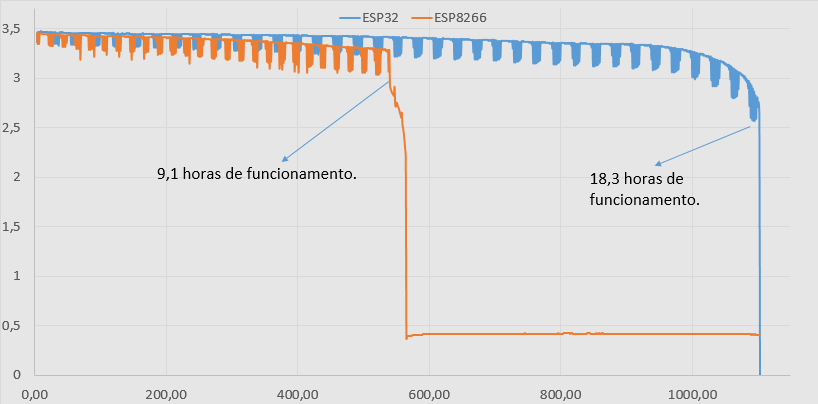
\includegraphics[scale = 0.7]{Graficos/grafico_02.png}
    \caption{Gráfico 2 - Comparativo entre ESP8266 e ESP32}
    \label{fig:grafico_results_02}
\end{figure}

{
Isso é provado a partir da comparação entre o gráfico 1 de consumo – figura \ref{fig:grafico_results_01}, no qual os ESPs não estão programados para realizar a troca de rotina de operações. Desse modo permanecem constantes sem alterar o modo de funcionamento. Por esse motivo não é perceptível nenhuma mudança abrupta no gráfico.
}

{
Devido a tal fato, a vida útil da bateria é fortemente danificada, pois não são preparadas para sofrerem esse tipo de variação de corrente elétrica, sendo percebível em todos os demais testes.
}

\begin{figure}[htp]
    \centering
    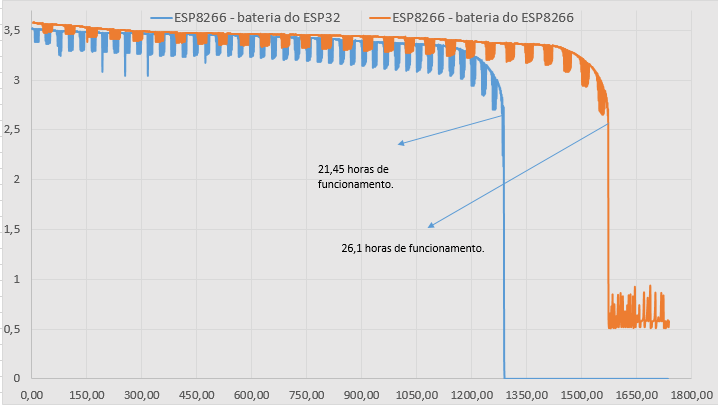
\includegraphics[scale = 0.8]{Graficos/grafico_03.png}
    \caption{Gráfico 3 - Segundo comparativo, mas com as baterias trocadas}
    \label{fig:grafico_results_03}
\end{figure}

\begin{figure}[htp]
    \centering
    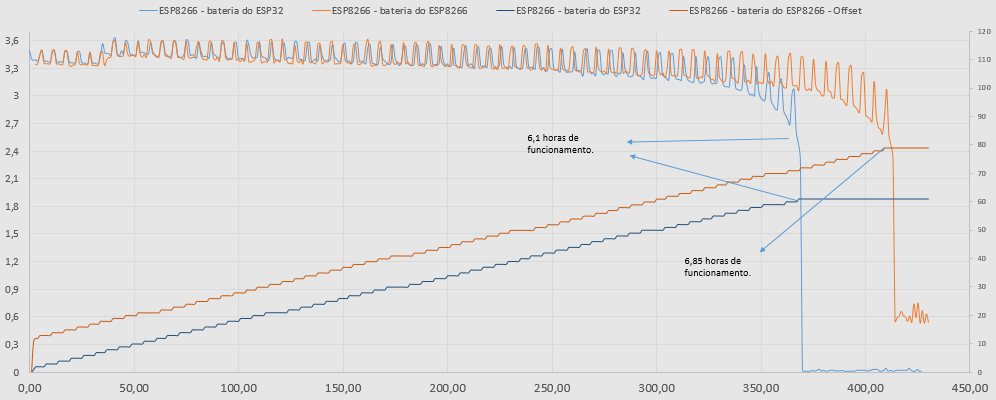
\includegraphics[scale = 0.6]{Graficos/grafico_04.png}
    \caption{Gráfico 4 - Comparativo com contador de ciclos}
    \label{fig:grafico_results_04}
\end{figure}

\begin{figure}[htp]
    \centering
    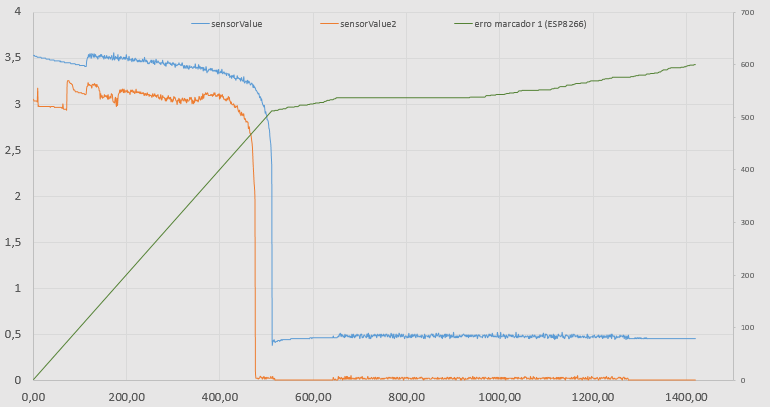
\includegraphics[scale = 0.7]{Graficos/grafico_05.png}
    \caption{Gráfico 5 - Ciclo sem Deep-Sleep ativo.}
    \label{fig:grafico_results_05}
\end{figure}

\begin{figure}[htp]
    \centering
    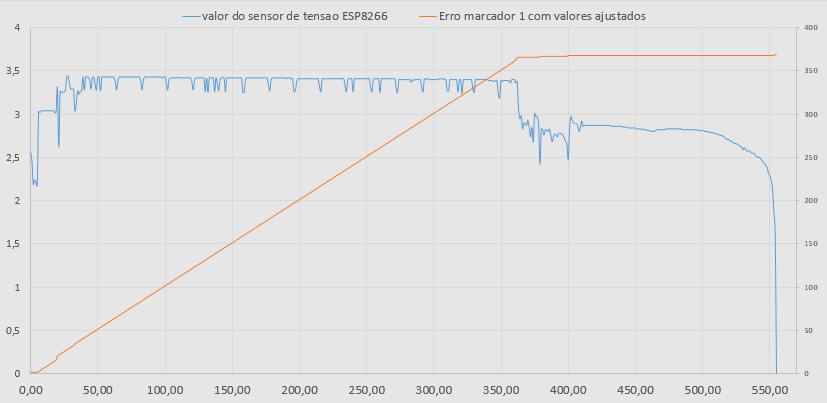
\includegraphics[scale = 0.7]{Graficos/grafico_06.png}
    \caption{Gráfico 6 - Análise de limiar de tensão para funcionamento da placa ESP8266}
    \label{fig:grafico_results_06}
\end{figure}

